%!TEX root = ../fbi.tex

\section{Construction of the featuresless boson insulator}

In Ref.~\onlinecite{kimchi2013}, Kimchi et al gave an explicit construction of a bosonic insulator
on the honeycomb lattice that is completely featureless in the bulk. The state is succinctly described by the following
wavefunction:
\begin{equation} \label{eq:def}
\ket{\psi} = \prod\limits_{\varhexagon} \sum\limits_{i \in \varhexagon} b^{\dagger}_{i} \ket{0}.
\end{equation}
Here, $\varhexagon$ denotes the elementary hexagons of the honeycomb lattice. We consider two closely related
variants of the state, a version of soft-core bosons where $b_i^\dagger$ creates a boson on site $i$ and obeys the
usual bosonic commutation relations, and a hard-core version of the same state where $b_i^\dagger$ also creates a
boson but $(b_i^\dagger)^2=0$.
In either case, the operator $\sum_{i \in \varhexagon} b^{\dagger}_{i}$ creates exactly one boson per hexagon;
as there is one hexagon per unit cell of two sites of the lattice, the state has one boson per unit cell, or half a boson per site.
In the case of soft-core bosons, the maximum number of bosons per site is 3.

\begin{figure}[H]
	\centering
	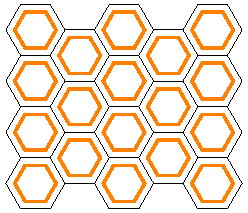
\includegraphics[width=0.6\columnwidth]{fbi3.pdf}
	\caption{Schematic representation of honeycomb FBI}
\end{figure}

\subsection{PEPS Construction of honeycomb F.B.I.}

In order to make the state~\eqnref{eq:def} more amenable to numerical simulations, and in particular in order to be able to study its
edge properties, we now derive a representation as a projected entangled pair states (PEPS). \bela{I would probably put the more
generic introduction to PEPS as generalization of MPS etc. in the Introduction rather than have it here.}
Importantly, this PEPS description will respect all of the relevant symmetries of \eqnref{eq:def}.

\begin{figure}[H]
	\centering
	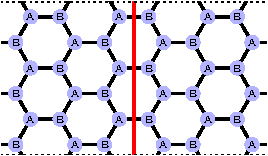
\includegraphics[width=\columnwidth]{Hex_PEPS.pdf}
	\caption{\bela{In this picture, we need to indicate the physical legs (maybe in a different color).} Pictoral representation of a PEPS on a honeycomb lattice. The tensors A and B are rank 4, with the physical leg at each site not shown for visual clarity. By gluing together the top and bottom edge of this picture, we get the "zig-zag" cylinder configuration used for most of the calculations in this paper. This cylinder is 3 unit cells wide, so we will call it the L=3 cylinder. In section \ref{sec:ES}, we will study the entanglement cut specified by the red line for various cylinder widths.}
	\label{fig:PEPS}
\end{figure}

\begin{figure}
	\centering
	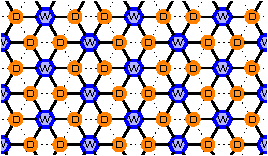
\includegraphics[width=0.8\columnwidth]{FBI_PEPS.pdf}
	\caption{\bela{Make labels math font. I think we might have to include physical indices in this figure, maybe very short/thin.}
	Intermediate tensor network for FBI state. Here, the tensors labeled $D$ are located on the
	sites of the honeycomb lattice, while the tensors labeled $W$ are located on the centers of each hexagon.
	Dotted lines thus represent the physical lattice, while the solid lines indicate auxiliary bonds over which the tensor network
	is contracted. In this picture, we have suppressed the physical index for visual clarity.}
	\label{fig:FBI_PEPS}
\end{figure}

To obtain a PEPS construction, we first choose a local basis $\ket{n}$ of boson occupation numbers, i.e. $b^\dagger b \ket{n} = n \ket{n}$. The
PEPS will thus describe the coefficients of $\ket{\psi}$ in this basis, $\langle n_1 \ldots n_L | \psi \rangle$.
The PEPS representation is most easily obtained in a two-step construction, where we first construct the state shown in Fig.~\ref{fig:FBI_PEPS}.
Here, the tensor labeled $W=W^{n_1 \ldots n_6}$, which is placed in the center of each hexagon, is a rank-6 tensor given by
\begin{equation}
W^{\{n_x\}}  = \left\{ \begin{array}{lr}
													1  : & \sum\limits_x n_x = 1 \\
													0  : & \text{else}
													\end{array} \right. .
\end{equation}
This tensor describes the coefficients of a so-called $W$-state in the occupation number basis, i.e. $W^{\lbrace n_x\rbrace }= \langle n_1 \ldots n_6 | \sum_{i=1}^6 b_i^\dagger |0\rangle$. We note that this tensor is symmetric under permutations of its indices.

On the sites of the physical lattice, we have placed a rank-4 tensor denoted as $D$ which connects the $W$ tensors from three adjacent hexagons,
and as fourth index has a physical index $p$. For a state of soft-core bosons, where $p=0,1,2,3$, this tensor is given by
\begin{equation} \label{eqn:D}
D^\mathrm{sc}_{p i_0 i_1 i_2}  = \left\{ \begin{array}{ll}
													\sqrt{p!}  &: p =i_0+i_1+i_2  \\
													0  &:  \text{else}
													\end{array}
											\right. .
\end{equation}
We can also encode a state of hard-core bosons by replacing $D$ by
\begin{equation}
D^\mathrm{hc}_{p i_0 i_1 i_2}  = \left\{ \begin{array}{ll}
													1  &: i_0+i_1+i_2 > 0  \\
													0  &:  \text{else}
													\end{array}
											\right. .
\end{equation}

%We can represent (\ref{eq:def}) as a tensor network by replacing the sum over each plaquette with a tensor contraction. The matrix elements of the plaquette boson creation operator can be specfied by a trace over one virtual qubit per site $x$ adjacent to the plaquette, as in 
%\begin{equation}
%\braopket{\{\alpha_x\}}{\sum\limits_{x \in \varhexagon} b^{\dagger}_{x}}{\{\beta_x\}} =
% \sum\limits_{\{i_x\}} W^{i_1 i_2 ... i_6} \prod\limits_x B^{i_x}_{\alpha_x \beta_x} 
%\label{eq:plaquette}
%\end{equation}
%
%in which the application of the creation operator at $x$ is controlled by the state of the virtual qubit $i_x$:
%\begin{equation*}
%B^i_{\alpha \beta} = \left\{
%     \begin{array}{lr}
%       \delta_{\alpha \beta} & : i = 0\\
%       (b^{\dagger})_{\alpha \beta} & : i = 1
%     \end{array}
%   \right\}.
%\end{equation*}
%
%The tensor $W^{i_0 i_1 i_2 i_3 i_4 i_5}$ should be taken as the W-state: 
%$$ W^{\{i_x\}}  = \left\{ \begin{array}{lr}
%													1  : & \sum\limits_x i_x = 1 \\
%													0  : & \text{else}
%													\end{array}
%											\right\} = \ket{100000} + ...\ket{000001}.
%$$
%
%By applying the operator to all plaquettes, we get a tensor network not in the form of Figure \ref{fig:PEPS}, but instead one with the rank 6 tensor $W$ located on each plaquette and a rank $3+1$ tensor $D$ located on the vertices, as shown in \ref{fig:FBI_PEPS}. 
%
%It is straightforward to show that the tensor $D^p_{ijk}$ should be
%$$
%D_{p}^{i_0 i_1 i_2} = \sum\limits_{\alpha \beta} B^{i_0}_{p \alpha}B^{i_1}_{\alpha \beta} B^{i_2}_{\beta 0}  = \left\{ \begin{array}{lr}
%													\sqrt{p!}  : & p =i_0+i_1+i_2  \\
%													0  : & \text{else}
%													\end{array}
%											\right\}
%$$
%to reproduce the action of the plaquette operators adjacent to each vertex. The boson number at the vertex $p$ can be limited to be $0, 1, 2,$ or $3$ since at most one boson comes from each of the three adjacent hexagons.

This tensor network wavefunction in this form manifestly has all the translational and point group symmetries of the honeycomb lattice, since the tensors $W$ and $D$ are invariant under rotations of their virtual indices in the plane, as shown in the picture. One can also check that the wavefunction is $U(1)$ invariant; all terms in the wavefunction are configurations with boson number exactly $1$ per plaquette.

In order to form a PEPS representation with all tensors located on the vertices, we can factor the W-state tensor and regroup the factors into PEPS tensors $A$ and $B$, as shown in Figure \ref{fig:FBI_PEPS_2}. 
There is a choice of MPS for the W-state that doesn't manifestly preserve the rotational symmetry the plaquettes, but has the small bond dimension $2$. (A different choice could be made that has bond dimension 6 but does preserve the symmetry.) This factorization of the W-state is given by

$$
W^{i_0 i_1 i_2 i_3 i_4 i_5} = \sum\limits_{abcde} W^{i_0 a}_{1} W^{i_1 b}_{a} W^{i_2 c}_{b} W^{i_3 d}_{c} W^{i_4 e}_{d} W^{i_5 0}_{e},
$$
where 
$$ W^{i_0 i_1}_{j}  = \left\{ \begin{array}{lr}
													1  : & i_0+i+1 = j \\
													0  : & \text{else}
													\end{array}
											\right\},
$$
and where each index takes values in $\{0, 1\}$. We will discover that the virtual edges in this PEPS can be assigned consistent $U(1)$ charges, with the index $i_x$ representing the charge. The arrows on the tensors show the flow of charge.

The rewriting of the tensor network does not change the physical wavefunction or physically invariant quantities, such as the Schmidt spectrum for the entanglement cut. However, it is computationally convenient - the total bond size crossed by the entanglement cut in Figure \ref{fig:PEPS} is $2^L$ for the cylinder of width $L$.

\begin{figure}[H]
	\centering
	\subfigure[W-state tensor and factored form]{%
		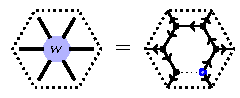
\includegraphics[width=0.6\columnwidth]{w_string.pdf}
		\label{fig:W}
	}
	\quad
	\subfigure[D tensor]{%
		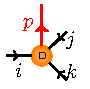
\includegraphics[width=0.3\columnwidth]{D_op.pdf}
		\label{fig:D}
	}
	\subfigure[PEPS tensor network for F.B.I. state]{%
		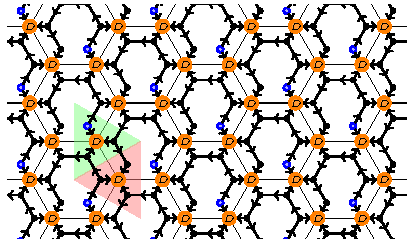
\includegraphics[width=0.8\columnwidth]{FBI_PEPS_2.pdf}
		\label{fig:FBI_PEPS_2A}
	}
		
%
\caption{\bela{I think the 1 in the center of the W MPS is confusing. Also, we should have shaded circles showing what the final PEPS tensor is.} Tensors used to put the F.B.I. tensor network in PEPS form. }
\label{fig:FBI_PEPS_2}
\end{figure}

%\begin{figure}[H]
%	\begin{columns}{t}
%	\begin{column}{width=0.25\textwidth]
%	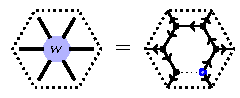
\includegraphics[width=0.6\columnwidth]{w_string.pdf}
%	\end{column}
%	\begin{column}{width=0.25\textwidth]
%	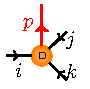
\includegraphics[width=0.6\columnwidth]{D_op.pdf}
%	\end{column}
%	\end{columns}
%\end{figure}
